\documentclass[]{report}
\usepackage{graphicx}

% Title Page
\title{AR Mirror Game user manual}
\author{Tim van Rossum}


\begin{document}
\maketitle
\section*{Starting up the server}
Before one can start up the server and actually have it do something, the master
camera needs to be connected to the computer that the server should run on. 
Then, the user should select whether completely red markers or red-and-yellow
markers should be detected as corner markers. They should also enter the camera
device ID (usually 1, if the computer has its own webcam, but it can also be 0.
It is advised to try out both options to find the one that works). The server
port and camera resolution can also be specified (the default server port is 
23369, and it is advised to not change it as that also has to be changed
client-side in that case). Enabling "Require empty board" will require the board
to be empty (no markers on the board) before the server can send any useful
information.\\
\\
The server UI also specifies some useful information: it shows the FPS the
server is recording the board at, the index of the current level, and a debug
overlay (if enabled) that shows what the camera sees, with marker indices
overlaid on the different markers.
\begin{figure}[!ht]
	\centering
	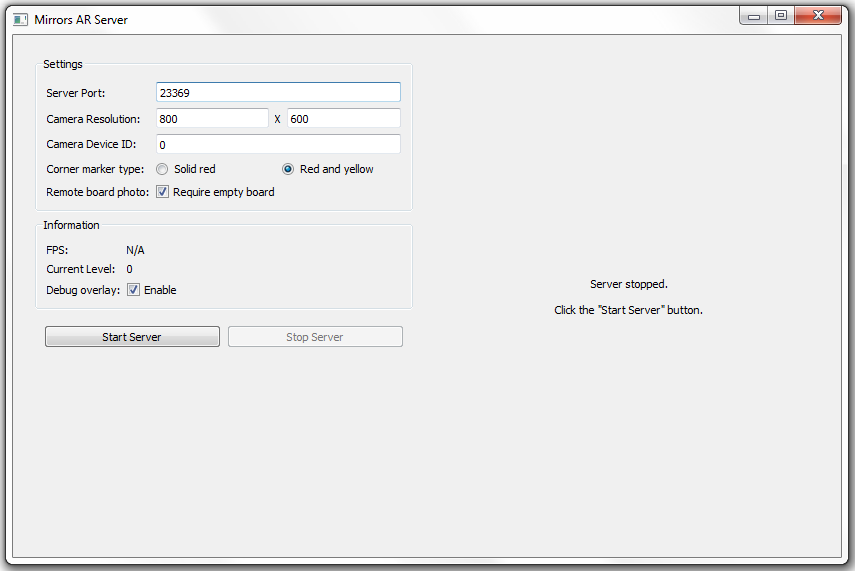
\includegraphics[scale = 0.5]{MirrorServerUI}
	\caption{The use cases for the remote player.}
\end{figure}
\end{document}          
